\subsection{Beschreibung der Komponenten}
Dieser Abschnitt beschreibt die physikalischen Komponenten, die von der Teilgruppe Materialfluss verwendet wurden. Zu den diesen Komponenten zählen die Rampen, sowie die \textsc{Mica}z-Module mit ihren Mikrocontrollern. 
\subsubsection{Rampen}
Rampen stellen Ein- und Ausgänge, sowie Zwischenlager im physischen System dar. Auf einer Rampe finden bis zu vier Pakete Platz. Bolzen hinter dem ersten Paket, separiert dieses von den anderen Dreien. Damit das vorderste Paket nicht vorne von der Rampe herunterfällt, sind an der Vorderseite zwei weitere Bolzen angebracht. 

Durch vier Lichtschranken, wird eine Überwachung der Rampe ermöglicht. Diese beinhaltet zum einen das Abfragen, wie viele Pakete auf einer Rampe liegen. Zum anderen kann durch die Überwachung überprüft werden, an welcher Stelle Pakete liegen.

Alle vier Bolzen sind seitlich der Rampe befestigt. Eine autonome Steuerung der Rampen, wird durch ein angebrachtes \textsc{Mica}z-Modul ermöglicht.
\autoref{fig:skiram} zeigt ein Beispiel solch einer Rampe.

\begin{figure}[h!]
	\centering
		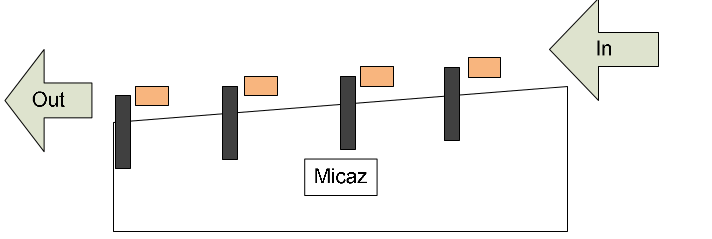
\includegraphics[width=0.9\textwidth]{SkizzeRampe.png}
	\caption{Beispiel einer eingesetzten Rampe}
	\label{fig:skiram}
\end{figure}

\subsubsection{Mikrocontroller}
Ein Mikrocontroller ist ein vollständiger Kleinstrechner auf einem einzigen Chip, dessen Zentraleinheit aus einem oder mehreren Mikroprozessen besteht. Zusätzlich enthält ein Mikrocontroller Speicher und Ein- bzw. Ausgabeschnittstellen zur Außenwelt. Dazu können neben einfach Ausgangspins auch komplexere Busprotokolle wie etwa USART, SPI oder CAN gehören.

Mikrocontroller werden eingesetzt, wenn eine Kommunikations- oder Steuerungsaufgabe mit möglichst geringen Ressourcen (Baugröße, Energie, Kosten) gelöst werden müssen. Die in einem Mikrocontroller verbauten Prozessorkern, Speicher und die Aus- und Eingabeschnittstellen, sind auf die Lösung derartiger Aufgaben zugeschnitten. Die große Anzahl an potenziellen Aufgabenstellungen hat zur Folge, dass es eine Vielfalt von Mikrocontrollern gibt. Meist sind die Mikrocontroller deshalb in Mikrocontrollerfamilien aufgeteilt. Innerhalb einer Familie unterscheiden sich die Controller nicht im Prozessorkern, sondern im verfügbaren Speicher und in den Ein- und Ausgabeschnittstellen \cite{ECHT2005}. In \autoref{fig:aufbmc} ist der schematische Aufbau eines MCs dargestellt.
\begin{figure}[th]
	\centering
		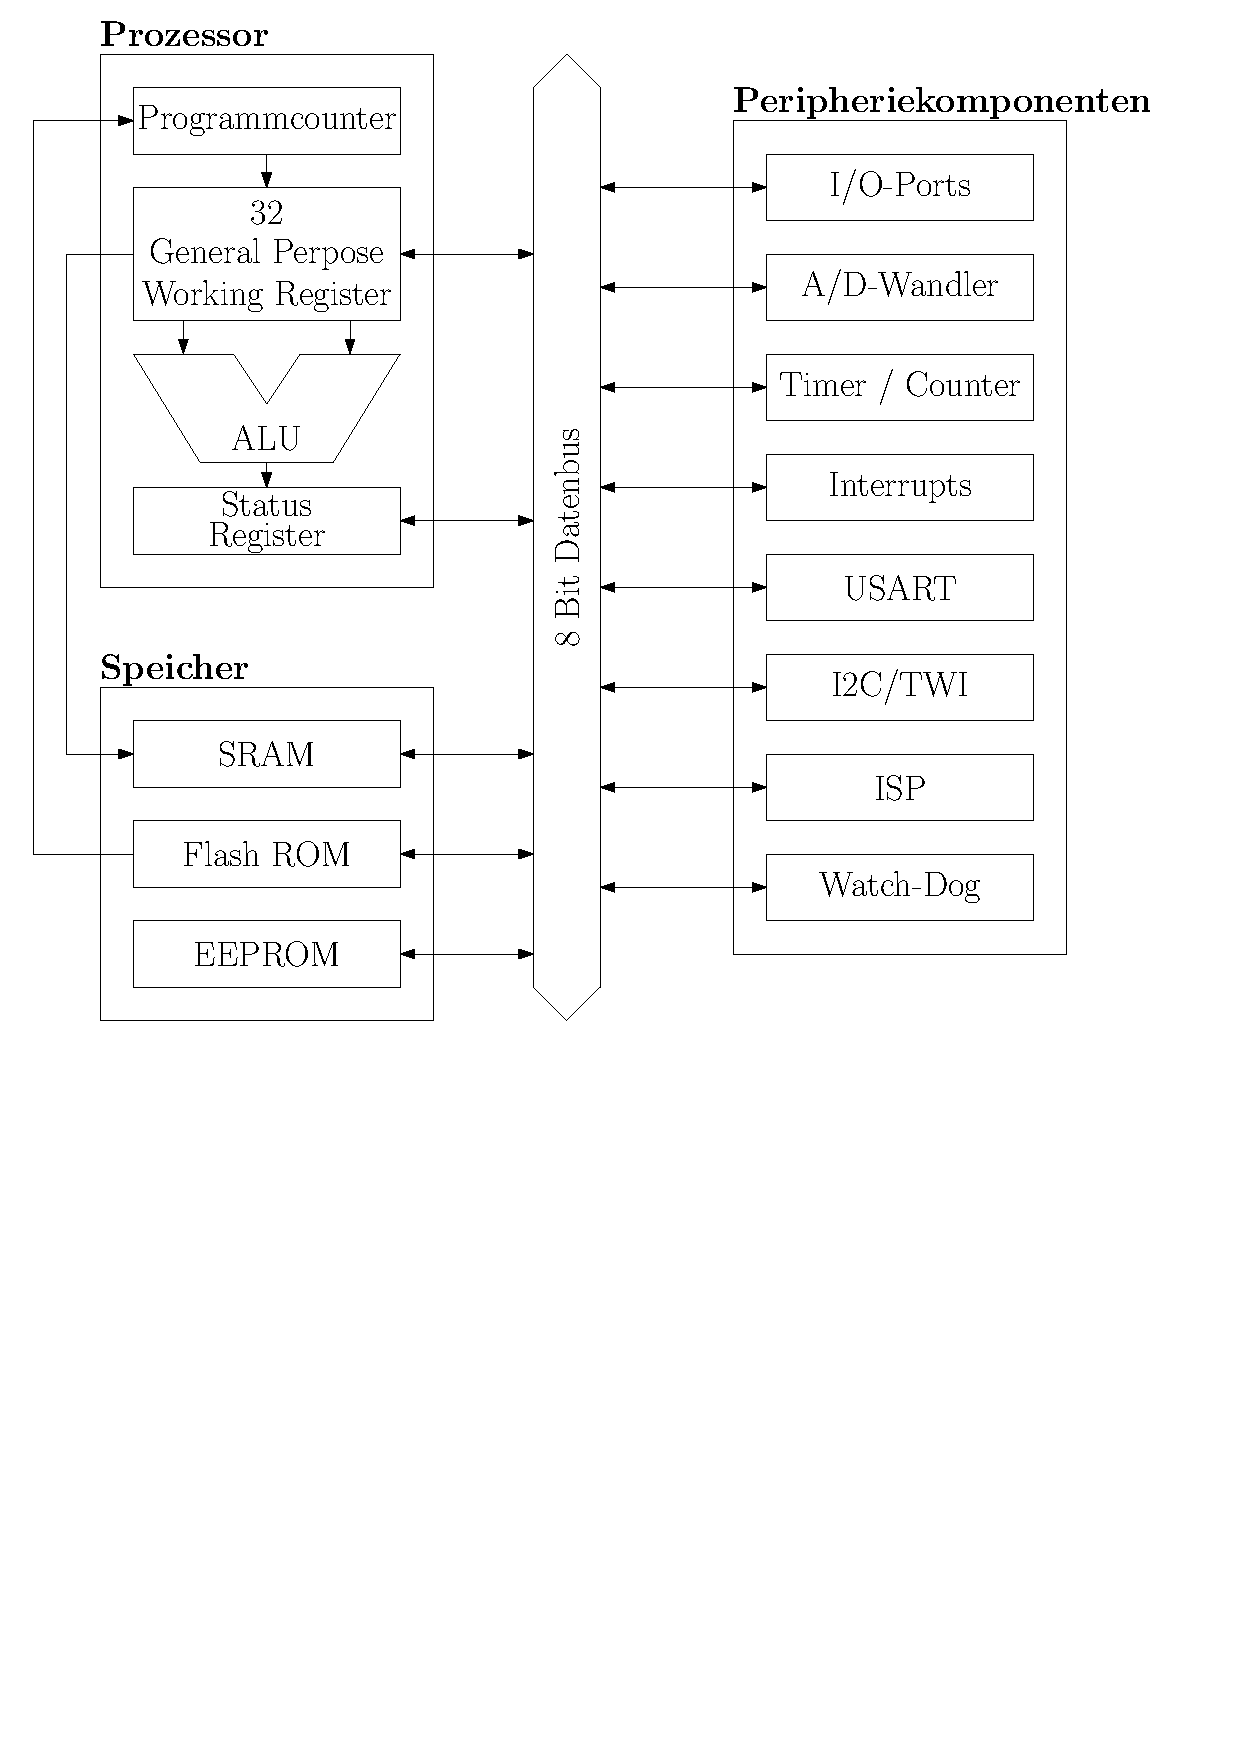
\includegraphics[width=0.8\textwidth]{flow/schemamc.pdf}
	\caption{Schematischer Aufbau eines Mikrocontrollers vgl. \cite{Brinkschulte:2002:Mikrocontroller}}
	\label{fig:aufbmc}
\end{figure}

Die zentrale Steuereinheit eines MCs ist der \textbf{Prozessor} (engl.: Central Processing Unit (CPU)). Sie ist die wichtigste Funktionseinheit und für die Verarbeitung von Befehlen und arithmetischen Berechnungen verantwortlich. Über den internen Bus kann die CPU mit weiteren Grundbausteien kommunizieren und beispielsweise auf Daten innerhalb des Speichers zugreifen.

Der \textbf{Speicher} besteht in der Regel aus dem Arbeitsspeicher (RAM, kurz für: Random Access Memory) und dem Programmspeicher bzw. Flash-Speicher. Normalerweise werden diese zwei Speichertypen logisch voneinander getrennt. Programme werden im nichtflüchtigen Flash-Speicher gesichert. Dieser kann mehrere Kilobyte (KB) bis Megabyte (MB) umfassen. Bei speziellen Systemen ist es möglich den Programmspeicher durch externe Flash-Komponenten zu erweitern um zusätzlichen Speicherplatz zu gewinnen.

Zwischenergebnisse, Messwerte von Sensoren, Steuergrößen usw. werden auf dem RAM abgelegt. Dieser ist deutlich schneller als der Flash-Speicher, verfügt aber in der Regel über deutlich weniger Speicherplatz. Alle Werte, welche zur Laufzeit im RAM abgelegt werden, sind im Gegensatz zum Flash-Speicher flüchtig. Das bedeutet, dass Daten bei einem Neustart des Mikrocontrollers nicht erhalten bleiben.

Durch die \textbf{Peripheriekomponenten} wird die Verbindung und Kommunikation zwischen Controller und Außenwelt ermöglicht. Über die digitalen Ein- und Ausgänge (GPIO, kurz für: General Purpose Input/Output) können Sensoren, Aktoren oder andere Systeme mit dem Mikrocontroller verbunden werden. Die meisten Mikrocontroller bieten eine Vielzahl von Ein- und Ausgängen \cite[S. 13-16]{SOM2012}.

Bei der Umsetzung des Projekts wurden \textsc{Mica}z-Module eingesetzt. Im Folgenden werden kurz die Eigenheiten dieser Module erläutert.

\begin{figure}[th]
  \centering
    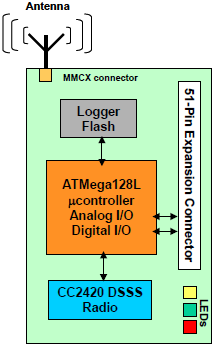
\includegraphics[width = 0.5\textwidth]{flow/blockmicaz.PNG}
    \caption{Blockdiagramm der \textsc{Mica}z-Module}
    \label{fig:blockmicaz}
\end{figure}

\paragraph{\textsc{Mica}z-Modul}
Abbildung \autoref{fig:blockmicaz} stellt ein Blockdiagramm der \textsc{Mica}z-Module dar. Herzstück der Module ist ein ATMega128L-Mikrocontroller. Bei diesem handelt es sich um einen Low-Power-Mikrocontroller von der Firma Atmel. Darüber hinaus verfügt ein \textsc{Mica}z-Module über einen CC2420-Funkchip der Firma Texas Instruments. Dieser ermöglicht die drahtlose Kommunikation mit anderen Modulen auf einer Frequenz von 2.4 GHz ermöglicht. Es wird dabei der IEEE 802.15.4 Standard verwendet. Eine Antenne kann über eine MMCX-Schnittstelle mit dem Modul verbunden werden, um Signalstärke und -reichweite zu erhöhen. Weiter verfügen die Module über einen 128 KB großen Flash-Speicher.
Zugang zu einee Vielzahl der Leitungen des Moduls gewährt ein 51-poliger Steckverbinder. Über eine Erweiterungsplatine werden so etwa die Lichtschranken und Magnetbolzen der Rampe angeschlossen. Denkbar wäre auch ein größerer Arbeitsspeicher, alle nötigen Pins des Mikrocontrollers sind über den Steckverbinder erreichbar.
Im Projekt wurde die Steckverbindung weiterhin dafür genutzt, die \textsc{Mica}z-Module über ein \textsc{Mib}520 an einen PC anzuschließen, um sie über eine UART-Schnittstelle auszulesen und per JTAG zu programmieren \cite{MICSHEET,C2420SHEET}.

\paragraph{\textsc{Mib}520}
Ein \textsc{Mib}520 stellt eine Schnittstelle für \textsc{Mica}z-Module dar. Es erlaubt die Verbindung eines \textsc{Mica}z-Moduls mit einem Computer per USB-Schnittstelle. So kann über die USART-Schnittstelle des Moduls mit dem PC kommuniziert werden. Über diese Verbindung wurde die Schnittstelle zu den Volksbots realisiert. Weiterhin verfügt ein \textsc{Mib}520-Gateway über eine \textbf{JTAG}-Schnittstelle. \textbf{JTAG} steht für \textit{Joint Test Action Group} und ist eine standardisierte (IEEE 1149.1, siehe \cite{IEEE1149:2014:Online}) Schnittstelle für das Programmieren und das Debuggging von integrierten Schaltungen.
%\paragraph{Sensorik und Aktorik}
%Hauptziel der Teilgruppe Materialfluss ist das Management von Paketen auf einer Rampe.
%Die Aufgabe der Sensorik ist dabei, dass die mit Lichtschranken ausgestatteten Rampen Pakete detektieren und auf Änderungen der Positionen der Pakete reagieren.
%Die Lichtschranken bestehen aus einer Lichtstrahlenquelle (dem Sender) und einem Sensor (dem Empfänger) f\"{u}r diese Strahlung.
%Als Lichtquelle kommt Infrarotlicht zum Einsatz und der Vorteil besteht in der einfachen Einstellung des Sensorsystems durch den
%sichtbaren Lichtfleck. Das Funktionsprinzip der Lichtschranke besteht darin, den sich  ändernden Zustand durch die Lichtintensität mit dem Sensor zu registrieren. 
%Die Rampen werden auf Hardwareebene um eine Aktorik zum Arretieren der Kisten ergänzt. Diese Aktoren (in unserem Fall die
%eingesetzte Bolzenpaare) sind für das Ausführen von Bewegungen zuständig.
%Sie sind aktive Stellelemente, die in der Antriebs- und Steuerungstechnik vom  Mikrorechner angesteuert werden, um das Verhalten des Prozesses durch das vom Sensor kommende Signal in einer gew\"{u}nschten Weise zu ermöglichen. In dieser allgemeinen Darstellung stehen die 
%Ausgangssignale eines Sensors und die Stellsignale der Aktoren mit einem
%Informationsverarbeitungssystem (IVS) in Verbindung.
